\documentclass{beamer}
\usepackage{alltt}
\usepackage{tikz}
\usetikzlibrary{matrix}
\usetikzlibrary{trees}
\usepackage{cancel}
\usepackage{subcaption}
\PassOptionsToPackage{obeyspaces}{url}
\usepackage{hyperref}
\usepackage{adjustbox}

\usepackage{lipsum}

\usetheme{Hannover}

\newcommand{\racket}{\texttt{Racket}}
\newcommand{\drr}{\texttt{DrRacket}}
\newcommand{\fsm}{\texttt{FSM}}
\newcommand{\ide}{\texttt{IDE}}
\newcommand{\api}{\texttt{API}}
\newcommand{\arrow}{\(\rightarrow\)}
\newcommand{\dotss}{\(\ldots\)}
\newcommand{\vdotss}{\(\vdots\)}
\newcommand{\elist}{\texttt{\textquotesingle{()}}}
\newcommand{\logand}{\texttt{\(\wedge\)}}
\newcommand{\logor}{\texttt{\(\vee\)}}
\newcommand{\imp}{\texttt{\(\Rightarrow\)}}
\newcommand{\sig}{\texttt{\(\Sigma\)}}
\newcommand{\delt}{\texttt{\(\delta\)}}
\newcommand{\sigsig}{\texttt{\(\Sigma\) = \{a b\}}}
\newcommand{\gam}{\texttt{\(\Gamma\)}}
\newcommand{\ep}{\texttt{\(\epsilon\)}}
\newcommand{\quot}{\texttt{\textquotesingle{}}}
\newcommand{\dquot}{\texttt{"}}
\newcommand{\qquot}{\texttt{\textasciigrave{}}}
\newcommand{\lambexpr}{\texttt{$\lambda$}-expression}
\newcommand{\lamb}{\texttt{$\lambda$}}
\newcommand{\is}{\texttt{::=}}

\definecolor{darkgreen}{RGB}{102,170,102}

\begin{document}

\title{Part II: Data Abstraction}
%\subtitle{Using Beamer}
\author{Marco T. Moraz\'{a}n}
\institute{Seton Hall University}
\date{}

\begin{frame}
\titlepage
\end{frame}

\begin{frame}
\frametitle{Outline}
\tableofcontents
\end{frame}

\section{Interface and Implementation}

\begin{frame}[fragile]
\frametitle{Definition and Implementation}
%\framesubtitle{HOMEWORK}
\begin{scriptsize}
\begin{itemize}
\item<1-> Representing a set means defining a new data type

\item<2-> Values are the representations

\item<2-> Operations are procedures that manipulate them

\item<3-> Data abstraction divides a data type in two pieces: interface and implementation

\item<4-> Interface
\begin{itemize}
  \item what the data type represents
  \item what the operations on the data are
  \item what properties these operations have
\end{itemize}

\item<5-> Implementation
\begin{itemize}
  \item provides a specific representation of the data
  \item provides code for the operations
\end{itemize}

\item<6-> Using abstract data types
\begin{itemize}
  \item Program manipulates data only through the defined operations
  \item Changing the representation only requires changing how the implementation of the operations in the interface; program that use the data types are unchanged
\end{itemize}

\end{itemize}
\end{scriptsize}
\end{frame}

\begin{frame}[fragile]
\frametitle{Definition and Implementation}
%\framesubtitle{HOMEWORK}
\begin{scriptsize}
\begin{itemize}
\item<1-> Idea is well-known to you
\begin{itemize}
  \item numbers: add, subtract, multiply, etc.
  \item files: open, close, save, etc.
\end{itemize}

\item<2-> OOP
\begin{itemize}
  \item Classes implement interfaces
  \item Programs use classes to declare and manipulate objects
\end{itemize}

\item<3-> The \emph{most important} part of an implementation is the \emph{specification of how data is represented}

\item<3-> $|$v$|$ denotes the representation of data v

\end{itemize}
\end{scriptsize}
\end{frame}

\begin{frame}[fragile]
\frametitle{Definition and Implementation}
\framesubtitle{Nonnegative Integers}
\begin{scriptsize}
\begin{itemize}
\item<1-> Interface
\begin{itemize}
  \item zero = $|$0$|$
  \item (isZero? $|$n$|$), \#t if n = 0 and \#f if n $\neq$ 0
  \item (succ $|$n$|$) = $|$n + 1$|$, n $\geq$ 0
  \item (pred $|$n + 1$|$) = $|$n$|$, n $\geq$ 0
  \item (dec2nnint $|$n$|_{10}$) = $|$n$|$
  \item (nnint2dec $|$n$|$) = $|$n$|_{10}$
\end{itemize}

\item<1-> No details on how nonnegative integers are represented

\item<1-> Only requires that procedures produce the desired behavior

\item<2-> Write a program to add to nonnegative integers

\item<3->
\begin{alltt}
;; nnint nnint \arrow{} nnint
;; Purpose: Add the given nnints
(define (plus x y)
  (if (isZero? x)
      y
      (succ (plus (pred x) y))))

(check-equal? (nnint2dec (plus (dec2nnint 0) (dec2nnint 0))) 0)
(check-equal? (nnint2dec (plus (dec2nnint 2) (dec2nnint 0))) 2)
(check-equal? (nnint2dec (plus (dec2nnint 0) (dec2nnint 1))) 1)
(check-equal? (nnint2dec (plus (dec2nnint 3) (dec2nnint 2))) 5)
\end{alltt}

\end{itemize}
\end{scriptsize}
\end{frame}

\begin{frame}[fragile]
\frametitle{Definition and Implementation}
\framesubtitle{Nonnegative Integers}
\begin{scriptsize}
\begin{itemize}
\item<1-> Unary Representation

\item<2->
\begin{alltt}
;; An nnint is either: 1. \elist{}  2. (cons \#t nnint)
\end{alltt}

\item<3->
\begin{alltt}
;; Constructors
;;  \arrow{} nnint
;; Purpose: Construct zero
(define (zero) \elist{})
\end{alltt}

\item<4->
\begin{alltt}
;; number \arrow{} nnint
;; Purpose: Construct nnint for the given decimal nnint
(define (dec2nnint n) (build-list n (lambda (i) \#t)))
\end{alltt}

\item<5->
\begin{alltt}
;; nnint \arrow{} nnint
;; Purpose: Construct the successor of the given nnint
(define (succ n) (cons \#t n))
\end{alltt}

\item<6->
\begin{alltt}
;; Observers
;; nnint \arrow{} Boolean
;; Purpose: Determine if given nnint is zero
(define (isZero? n) (null? n))
\end{alltt}

\item<7->
\begin{alltt}
;; nnint \arrow{} nnint
;; Purpose: Return the predecessor of given nnint
(define pred cdr)
\end{alltt}

\item<8->
\begin{alltt}
;; nnint \arrow{} number
;; Purpose: Return decimal representation of given nnint
(define (nnint2dec n) (length n))
\end{alltt}

\end{itemize}
\end{scriptsize}
\end{frame}

\begin{frame}[fragile]
\frametitle{Definition and Implementation}
\framesubtitle{Nonnegative Integers}
\begin{scriptsize}
\begin{itemize}
\item<1-> Racket Numbers Representation

\item<2->
\begin{alltt}
;; A nnint is a nonnegative Racket integer
\end{alltt}

\item<3->
\begin{alltt}
;; Constructors
;;  \arrow{} nnint    Purpose: Construct zero
(define (zero) 0)
\end{alltt}

\item<4->
\begin{alltt}
;; number \arrow{} nnint
;; Purpose: Construct nnint for the given decimal nnint
(define (dec2nnint n) n)
\end{alltt}

\item<5->
\begin{alltt}
;; nnint \arrow{} nnint
;; Purpose: Construct the successor of the given nnint
(define succ add1)
\end{alltt}

\item<6->
\begin{alltt}
;; Observers
;; nnint \arrow{} Boolean  Purpose: Determine if given nnint is zero
(define isZero? zero?)
\end{alltt}

\item<7->
\begin{alltt}
;; nnint \arrow{} nnint
;; Purpose: Return the predecessor of given nnint
(define (pred n)
  (if (= n 0)
      (eopl:error 'pred "Zero does not have a predecessor.")
      (sub1 n)))
\end{alltt}

\item<8->
\begin{alltt}
;; nnint \arrow{} number
;; Purpose: Return decimal representation of given nnint
(define (nnint2dec n) n)
\end{alltt}

\end{itemize}
\end{scriptsize}
\end{frame}

\begin{frame}[fragile]
\frametitle{Definition and Implementation}
\framesubtitle{Nonnegative Integers}
\begin{scriptsize}
\begin{itemize}
\item<1-> Bignum representation

\item<2-> Numbers are represented in base N (large N)

\item<2-> The representation uses a list of numbers such that each number is in 0..N-1 (called bigits)

\item<3-> Inductive Definition of $|$n$|$
\begin{equation*}
f(n)=\begin{cases}
       \elist{} & \text{if \(n=0\)} \\
       (cons \ r \ |q|) & \text{otherwise}, where n = q*N + r, 0 \leq r < N
     \end{cases}
\end{equation*}

\item<4-> N = 100

\item<4-> $|$131$|$ = (31 1)	

\item<4-> $|$87$|$ = (87)		

\item<4-> $|$6874$|$ = (74 68)

\item<5-> N = 500

\item<5-> $|$6874$|$ = (374  13) = 13*500 +374


\end{itemize}
\end{scriptsize}
\end{frame}

\begin{frame}[fragile]
\frametitle{Definition and Implementation}
%\framesubtitle{HOMEWORK}
\begin{scriptsize}
\begin{itemize}

\item<1-> QUIZ: 2.1, include nnint2dec and dec2nnint (Due in 1 week)

\end{itemize}
\end{scriptsize}
\end{frame}

\begin{frame}[fragile]
\frametitle{Environments}
%\framesubtitle{HOMEWORK}
\begin{scriptsize}
\begin{itemize}
\item<1-> An environment (env) associates a value with each element of a finite set of vars

\item<2-> Given a var an env returns its value

\item<2-> It's a function!

\item<3-> Interface (constructors and observers)
  \begin{itemize}
    \item (empty-env) = $|\varnothing|$, constructor
    \item (apply-env $|$e$|$ var) = e(var), observer
    \item (extend-env var v $|$e$|$) = $|$g$|$, constructor
    \begin{equation*}
      g(var1)=\begin{cases}
                v & \text{if \(var=var1\)} \\
                f(var1) & \text{otherwise}
              \end{cases}
    \end{equation*}
  \end{itemize}

\item<4-> (define e (extend-env  \quot{}x
				                  2
				                  (extend-env \quot{}y 1 (empty-env))))

\item<4-> (apply-env e \quot{}y) is ?

\item<4-> (apply-env e \quot{}x) is ?

\item<4-> (apply-env e \quot{}z) is ?


\end{itemize}
\end{scriptsize}
\end{frame}

\begin{frame}[fragile]
\frametitle{Environments}
%\framesubtitle{HOMEWORK}
\begin{scriptsize}
\begin{itemize}
\item<1-> Data Structure Representation

\item<1->
\begin{tabular}{lll}
  % after \\: \hline or \cline{col1-col2} \cline{col3-col4} ...
   $<$env$>$ & \is{} & (empty-env) \\
         & \is{} & (extend-env $<$symbol$>$ $<$Racket-value$>$ $<$env$>$) \\
\end{tabular}

\item<2->
\begin{alltt}
;;  \arrow{} env
;; Purpose: Construct the empty env
(define (empty-env) \quot{}(empty-env))
\end{alltt}

\item<3->
\begin{alltt}

;; symbol X env \arrow{} env
;; Purpose: Add a binding to the given env
(define (extend-env var val e)
  (list \quot{}extend-env var val e))
\end{alltt}

\item<4->
\begin{alltt}
;; env symbol \arrow{} X
;; Purpose: Get the value of given var in given env
(define (apply-env e var)
  (cond [(eq? (car e) \quot{}empty-env)
         (eopl:error \quot{}apply-env "No binding for ~s" var)]
        [(eq? (cadr e) var) (caddr e)]
        [else (apply-env (cadddr e) var)]))
\end{alltt}

\end{itemize}
\end{scriptsize}
\end{frame}

\begin{frame}[fragile]
\frametitle{Environments}
%\framesubtitle{HOMEWORK}
\begin{scriptsize}
\begin{itemize}
\item<1-> Procedural Representation

\item<1-> env instances must offer all the observers (cf. an object)

\item<2->
\begin{alltt}
(define (empty-env)
  (lambda (search-var)
    (eopl:error \quot{}apply-env "No binding for ~s" search-var)))
\end{alltt}

\item<3->
\begin{alltt}
(define (extend-env var val e)
  (lambda (search-var)
    (cond [(eqv? search-var var) val]
          [else (apply-env e search-var)])))
\end{alltt}

\item<4->
\begin{alltt}
(define (apply-env e var) (e var))
\end{alltt}

\end{itemize}
\end{scriptsize}
\end{frame}

\begin{frame}[fragile]
\frametitle{Environments}
%\framesubtitle{HOMEWORK}
\begin{scriptsize}
\begin{itemize}
\item<1-> HOMEWORK: 2.7-2.9

\item<2-> QUIZ: 2.12 (Due in 1 week)

\end{itemize}
\end{scriptsize}
\end{frame}

\begin{frame}[fragile]
\frametitle{Abstraction for Recursive Data}
%\framesubtitle{HOMEWORK}
\begin{scriptsize}
\begin{itemize}
\item<1->
\begin{tabular}{lll}
  % after \\: \hline or \cline{col1-col2} \cline{col3-col4} ...
   $<$bintree$>$ & \is{} & $<$number$>$ \\
         & \is{} & ($<$symbol$>$ $<$bintree$>$ $<$bintree$>$) \\
\end{tabular}

\item<1-> Defines the elements of the set as Racket values

\item<1-> This is a \emph{representation choice}

\item<2-> What should the interface look like?

\item<2-> Constructors to build each kind of $<$bintree$>$

\item<2-> a predicate to test if a value is a $<$bintree$>$

\item<2-> a way of distinguishing between a leaf and an internal node

\item<2-> a way of extracting its components


\end{itemize}
\end{scriptsize}
\end{frame}

\begin{frame}[fragile]
\frametitle{Abstraction for Recursive Data}
%\framesubtitle{HOMEWORK}
\begin{scriptsize}
\begin{itemize}
\item<1-> We will use: define-datatype

\item<2-> Syntax and Semantics
\begin{alltt}
(define-datatype type-name type-predicate-name
  {(variant-name { (field-name predicate)}\(\sp{*}\))}\(\sp{*}\))
\end{alltt}

\item<2-> can only be used at the top level

\item<2-> Creates a variant record data type named type-name

\item<2-> Each variant has a name and 0 or more fields

\item<2-> Each field has a name and associated predicate

\item<2-> No two types may have the same name

\item<2-> No two variants may have the same name even if they belong to different types

\item<2-> Each field predicate must be a one-argument function used to assure that the field’s values are valid

\end{itemize}
\end{scriptsize}
\end{frame}

\begin{frame}[fragile]
\frametitle{Abstraction for Recursive Data}
%\framesubtitle{HOMEWORK}
\begin{scriptsize}
\begin{itemize}
\item<1->
\begin{tabular}{lll}
  % after \\: \hline or \cline{col1-col2} \cline{col3-col4} ...
   $<$bintree$>$ & \is{} & $<$number$>$ \\
         & \is{} & ($<$symbol$>$ $<$bintree$>$ $<$bintree$>$) \\
\end{tabular}

\item<2->
\begin{alltt}
(define-datatype bintree bintree?
\end{alltt}

\item<3->
\begin{alltt}
  (leaf-node
    (datum number?))
\end{alltt}

\item<4->
\begin{alltt}
  (interior-node
    (key symbol?)
    (left bintree?)
    (right bintree?)))
\end{alltt}

\item<5-> Creates 1-argument function, bintree?, to test if something is a bintree

\item<5-> Creates a 1-argument function, leaf-node, to create a leaf; Argument is tested with number?. If it fails an error is reported

\item<5-> Creates a 3-argument procedure, interior-node, to create an interior node; First argument tested with symbol? and other 2 with bintree?

\end{itemize}
\end{scriptsize}
\end{frame}

\begin{frame}[fragile]
\frametitle{Abstraction for Recursive Data}
%\framesubtitle{HOMEWORK}
\begin{scriptsize}
\begin{itemize}
\item<1->
\begin{tabular}{lll}
  % after \\: \hline or \cline{col1-col2} \cline{col3-col4} ...
   $<$slist$>$ & \is{} & $<$(\{sexp\}$^*>$) \\
   $<$sexp$>$  & \is{} & $<$symbol$>$ \\
               & \is{} & $<$slist$>$ \\
\end{tabular}

\item<2->
\begin{alltt}
(define-datatype s-list s-list?
  (empty-s-list)
\end{alltt}

\item<3->
\begin{alltt}
  (non-empty-s-list
    (first s-exp?)   \textcolor{red}{creates its own list representation}
    (rest s-list?)))
\end{alltt}

\item<4->
\begin{alltt}
(define-datatype s-exp s-exp?
\end{alltt}

\item<5->
\begin{alltt}
  (symbol-symbol-exp (data symbol?))
\end{alltt}

\item<6->
\begin{alltt}
  (s-list-symbol-exp (data s-list?)) )
\end{alltt}

\end{itemize}
\end{scriptsize}
\end{frame}

\begin{frame}[fragile]
\frametitle{Abstraction for Recursive Data}
%\framesubtitle{HOMEWORK}
\begin{scriptsize}
\begin{itemize}
\item<1->
\begin{tabular}{lll}
  % after \\: \hline or \cline{col1-col2} \cline{col3-col4} ...
   $<$slist$>$ & \is{} & $<$(\{sexp\}$^*>$) \\
   $<$sexp$>$  & \is{} & $<$symbol$> |$  $<$slist$>$
\end{tabular}

\item<2->
\begin{alltt}
(define-datatype s-list s-list?
  (an-s-list  (data  (list-of symbol-exp?))))
(define (symbol-exp? e)
  (or (symbol? e) (and (pair? e) ((list-of symbol-exp?) e)))
\end{alltt}

\item<3->
\begin{alltt}
(define-datatype s-exp s-exp?
\end{alltt}

\item<4->
\begin{alltt}
  (symbol-symbol-exp (data symbol?))
\end{alltt}

\item<5->
\begin{alltt}
  (s-list-symbol-exp (data s-list?)) )
\end{alltt}

\end{itemize}
\end{scriptsize}
\end{frame}

\begin{frame}[fragile]
\frametitle{Abstraction for Recursive Data}
%\framesubtitle{HOMEWORK}
\begin{scriptsize}
\begin{itemize}
\item<1-> Write a program to sum the numbers in a bintree
\begin{alltt}
(define-datatype bintree bintree?
  (leaf-node (data number?))
  (interior-node (key symbol?)
                 (lst bintree?)
                 (rst bintree?)))
\end{alltt}

\item<2->
\begin{alltt}
;; Sample bintree
(define BT0 (leaf-node 4))
(define BT1 (interior-node \quot{}T (leaf-node 2) (leaf-node -2)))
(define BT2 (interior-node \quot{}T
                           (interior-node
                             \quot{}L (leaf-node 10) (leaf-node 20))
                           (interior-node
                             \quot{}L (leaf-node 30) (leaf-node 40))))
\end{alltt}

\item<3->
\begin{alltt}
;; bintree \arrow{} number
;; Purpose: Add nums in given bintree
(define (leaf-sum t)
\end{alltt}

\item<5->
\begin{alltt}
  (cases bintree t
    (leaf-node (val) val)
    (interior-node (k l r)
      (+ (leaf-sum l) (leaf-sum r)))))
\end{alltt}

\item<4->
\begin{alltt}
(check-equal? (leaf-sum BT0) 4)
(check-equal? (leaf-sum BT1) 0)
(check-equal? (leaf-sum BT2) 100)
\end{alltt}
\end{itemize}
\end{scriptsize}
\end{frame}

\begin{frame}[fragile]
\frametitle{Abstraction for Recursive Data}
%\framesubtitle{HOMEWORK}
\begin{scriptsize}
\begin{itemize}
\item<1->
\begin{tabular}{lll}
  $<$\textbf{exp}$>$ & \is{} & $<$number$>$ \\
            & \is{} & $<$Boolean$>$ \\
            & \is{} & $<$id$>$ \\
            & \is{} & (lambda ($<$id$>^*$) $<$exp$>$) \\
            & \is{} & ($<$exp$>$ $<$exp$>^*$) \\
    %\hline
\end{tabular}

\item<1-> A BNF grammar specifies a particular representation using specific strings and values

\item<1-> Called: \emph{Concrete Syntax} or External Representation

\item<2->
\begin{alltt}
(define-datatype \textbf{expr} expr?
  (var-expr (id symbol?))
  (num-expr (num number?))
  (bool-expr (b boolean?))
  (lambda-expr
   (params (list-of symbol?))
   (body expr?))
  (app-expr
   (op expr?)
   (args (list-of expr?))))
\end{alltt}

\item<2-> Called \emph{Abstract Syntax} or Internal Representation
	
\item<2-> Terminal symbols are not stored (e.g., keywords, ( and ))

\end{itemize}
\end{scriptsize}
\end{frame}

\begin{frame}[fragile]
\frametitle{Abstraction for Recursive Data}
%\framesubtitle{HOMEWORK}
\begin{scriptsize}
\begin{itemize}
\item<1-> An abstract syntax tree is created from an instance of concrete syntax through a process called \emph{parsing}

\item<1-> Each node corresponds to a step in the syntactic derivation

\item<1-> Internal nodes are named with a syntactic category

\item<1-> Edges are labeled with the names occurring in a syntactic category

\item<1-> Leaves correspond to terminal strings

\item<2-> ((lambda (x) (f x)) (g y))

\item<2->
\begin{center}
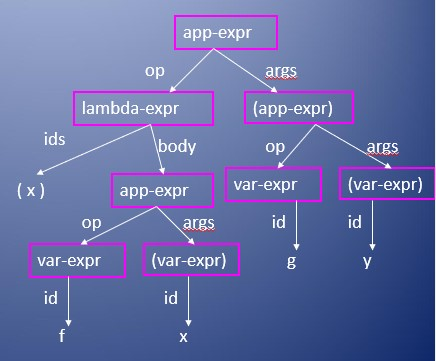
\includegraphics[scale=0.8]{lc-parse-tree.jpg}
\end{center}

\item<3-> Transforming an abstract syntax tree back to concrete syntax is called \emph{unparsing}

\end{itemize}
\end{scriptsize}
\end{frame}

\begin{frame}[fragile]
\frametitle{Abstraction for Recursive Data}
%\framesubtitle{HOMEWORK}
\begin{scriptsize}
\begin{itemize}
\item<1-> Abstract syntax trees are important

\item<1-> Programs that manipulate other programs are syntax oriented
compilers and interpreters (like Watson’s natural language parser and interpreter)

\item<1-> Transforming a program into a abstract syntax tree makes manipulating programs significantly easier
\end{itemize}
\end{scriptsize}
\end{frame}

\begin{frame}[fragile]
\frametitle{Environments}
%\framesubtitle{HOMEWORK}
\begin{scriptsize}
\begin{itemize}
\item<1->
\begin{alltt}
;; Sample exp (concrete syntax)
(define E0 \quot{}x)
(define E1 100)
(define E2 \#t)
(define E3 \quot{}(lambda (x y) (+ x y)))
(define E4 \quot{}((lambda (x y) (+ x z)) 2 3))

(check-equal? (unparse-lc-expr (parse-lc-exp E0)) E0)
(check-equal? (unparse-lc-expr (parse-lc-exp E1)) E1)
(check-equal? (unparse-lc-expr (parse-lc-exp E2)) E2)
(check-equal? (unparse-lc-expr (parse-lc-exp E3)) E3)
(check-equal? (unparse-lc-expr (parse-lc-exp E4)) E4)
\end{alltt}

\end{itemize}
\end{scriptsize}
\end{frame}

\begin{frame}[fragile]
\frametitle{Definition and Implementation}
%\framesubtitle{HOMEWORK}
\begin{scriptsize}
\begin{itemize}
\item<1->
\begin{alltt}
;; exp \arrow{} expr
;; Purpose: Parse the give LC exp
(define (parse-lc-exp e)
\end{alltt}

\item<2->
\begin{alltt}
  (cond [(symbol? e) (var-expr e)]
        [(number? e) (num-expr e)]
        [(boolean? e) (bool-expr e)]
\end{alltt}

\item<3->
\begin{alltt}
        [(eq? (car e) \quot{}lambda)
         (lambda-expr (cadr e)
                      (parse-lc-exp (caddr e)))]
\end{alltt}

\item<4->
\begin{alltt}
        [else (app-expr
               (parse-lc-exp (car e))
               (map (lambda (aexp) (parse-lc-exp aexp))
                    (cdr e)))]))
\end{alltt}

\item<5->
\begin{alltt}
;; expr \arrow{} exp
;; Purpose: Unparse the given LC expr
(define (unparse-lc-expr er)
\end{alltt}

\item<6->
\begin{alltt}
  (cases expr er
    (var-expr (s) s)
    (num-expr (n) n)
    (bool-expr (b) b)
\end{alltt}

\item<7->
\begin{alltt}
    (lambda-expr (params body)
                 (list \quot{}lambda params (unparse-lc-expr body)))
\end{alltt}

\item<8->
\begin{alltt}
    (app-expr (op args)
              (cons (unparse-lc-expr op)
                    (map (lambda (exr) (unparse-lc-expr exr))
                         args)))))
\end{alltt}

\end{itemize}
\end{scriptsize}
\end{frame}

\begin{frame}[fragile]
\frametitle{Definition and Implementation}
%\framesubtitle{HOMEWORK}
\begin{scriptsize}
\begin{itemize}
\item<1-> HOMEWORK: 2.21, 2.22, 2.24, 2.25, 2.27, 2.28, 2.29

\end{itemize}
\end{scriptsize}
\end{frame}


\end{document} 